\documentclass[12pt,letterpaper]{article}

\usepackage{amsmath} 
\usepackage{amssymb}
\usepackage{ulem}
\usepackage{tikz}
\usepackage[left=1in,top=1in,right=1in,bottom=1in,nohead]{geometry}
\usetikzlibrary{decorations.markings}
\usetikzlibrary{decorations.pathreplacing}

\usepackage{amsthm} 
\usepackage{wrapfig}
\usepackage{enumitem}
%\usepackage{enumerate}
\newtheorem{mydef}{Definition}
\newtheorem{example}{Example}
\newtheorem{thrm}{Theorem}
\newtheorem{lemma}{Lemma}
\newtheorem{cor}{Corollary}
\newtheorem{notation}{Notation}
\newtheorem{rem}{Remarks}
\newcommand{\biu}[1]{\underline{\textbf{\textit{#1}}}}
\newcommand{\so}{\Rightarrow}
\usepackage[ampersand]{easylist}

\let\oldemptyset\emptyset
\let\emptyset\varnothing

\newcommand{\homework}{\biu{Homework}}
\newcommand{\Mor}{\text{Mor}}
\newcommand{\N}{\mathbb{N}}
\newcommand{\Q}{\mathbb{Q}}
\newcommand{\Z}{\mathbb{Z}}
\newcommand{\R}{\mathbb{R}}
\newcommand{\C}{\mathbb{C}}
\newcommand{\pabs}[1]{\left|\left| #1 \right|\right|_p}
%\newcommand{\pabs}[1]{#1}
\begin{document}
\tikzstyle{lattice}=[shape=circle,draw,fill,text=white]
\tikzset{
  % style to apply some styles to each segment of a path
  on each segment/.style={
    decorate,
    decoration={
      show path construction,
      moveto code={},
      lineto code={
        \path [#1]
        (\tikzinputsegmentfirst) -- (\tikzinputsegmentlast);
      },
      curveto code={
        \path [#1] (\tikzinputsegmentfirst)
        .. controls
        (\tikzinputsegmentsupporta) and (\tikzinputsegmentsupportb)
        ..
        (\tikzinputsegmentlast);
      },
      closepath code={
        \path [#1]
        (\tikzinputsegmentfirst) -- (\tikzinputsegmentlast);
      },
    },
  },
  % style to add an arrow in the middle of a path
  end arrow/.style={postaction={decorate,decoration={
        markings,
        mark=at position 1 with {\arrow[#1]{stealth}}
      }}},
}



Consider two sets $X$ and $Y$ and let us define a relation R (between them) by $R \subseteq X \ Y$. For this it is convenient to use the notation $xRy$ which means $(x,y)\in R$

\begin{mydef}
For a relation $R$ with $X=Y$, we may define
\begin{description}
  	\item[$R_1$] \biu{reflexive} $xRx$ for every $x\in X$
    \item[$R_2$] \biu{symmetric} $x_1Rx_2\so x_2Rx_1 $
	\item[$R_3$] \biu{transitive}  $x_1Rx_2 \land x_2Rx_3 \so x_1Rx_3$
\end{description}
\end{mydef}

\begin{example}
\begin{minipage}{5in}
\begin{itemize}
\item $=$ is an equivalence relation (satisfying $R_1$-$R_3$)
\item $\leq$ on $\mathbb{R}$ is an ordered relation (satisfying $R_1$ and $R_3$
\end{itemize}
\end{minipage}
\end{example}

\begin{mydef} $X$ and $Y$ having the same cardinality if $\exists$ a map $F: X\to Y$ which is 1:1 (injective) and onto (surjective).
\end{mydef}

Intuitively $X$ and $Y$ have the "same cardinality" means they have the "same size".
The "same cardinality" relation satisfies $R_1$-$R_3$ is thus an equivalence relation. 

\begin{thrm}
\biu{Schr\"{o}der-Bernstein theorem}\newline
Suppose $X,Y$ are non-empty sets and $F: X\to Y$ and $G: Y\to X$ are injective maps. Then $X$ and $Y$ have the same cardinality.
\begin{proof}
Suppose $x\in X$, $x_0 \in X$, respectively $y_0\in Y$. \newline 
We shall say that $x_0$ is an \textbf{antecedent} of x of order $2n$, respectively $y_0$ is an antecedent of $x$ of order $2n-1$ if $x=(G\circ F)^n(x_0)$ and respectively $x=(G\circ F)^{n-1}G(y_0)$. Similarly for $y\in Y$.\newline
We will define 
\begin{eqnarray*}
 &X_{even} &= \left\{ x\in X | \text{ s.t. the "earliest antecedent" of } x \text{ has \underline{finite even} oder}\right\}\\
 &X_{odd} &= \left\{x\in X | \text{ s.t. the "earliest antecedent" of } x \text{ has \underline{finite odd} oder}\right\}\\
 &X_\infty &= \left\{x\in X | \text{ s.t. x has an infinite chain of antecedents}\right\}
\end{eqnarray*}

Then we construct the sets $X$ and $Y$ by taking the (disjoint) union over its parts:

\begin{align*}
X &= X_{even} \cup X_{odd} \cup X_\infty \\
Y &= Y_{even} \cup Y_{odd} \cup Y_\infty
\end{align*}

Let us now define $H$ as 

\begin{center}
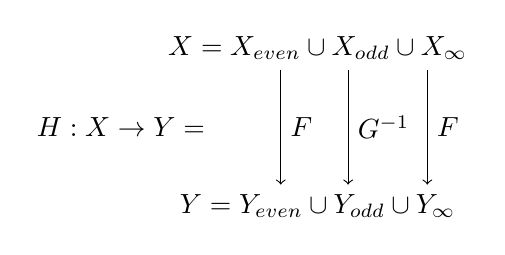
\begin{tikzpicture}[node distance=2cm, auto]
  \node (X) {$X = X_{even} \cup X_{odd} \cup X_\infty$};
  \node (Y) [below of=X] {$Y = Y_{even} \cup Y_{odd} \cup Y_\infty$};
  \node (H) at (-2.5cm,-1cm) {$H: X\to Y =$};
  \draw[->] (X.210) to node {$F$} (Y.150);
  \draw[->] (X.325) to node {$G^{-1}$} (Y.35);
  \draw[->] (X.349) to node {$F$} (Y.11);
\end{tikzpicture}
\end{center}

Clearly H is a bijective map (i.e. both injective and surjective) and thus by the definition of cardinality, we must have $card(X)=card(Y)$.

\end{proof}
\end{thrm}

\begin{lemma}
Suppose $F:X\to Y$ is a surjective map. Then there exists an injective map $G: Y\to X$ s.t. $(F \circ G): Y\to Y$ is the identity.
\end{lemma}
\begin{proof}
Suppose $y\in Y$. Then there exists $x \in X$ s.t. $F(x)=y$. Define $G(y)=x$. \newline \underline{\textbf{Note:}} This is one formulation of the axiom of choice.
\end{proof}
\begin{cor}
Suppose $X,Y$ are non-empy setes. Then the following are equivalent.
\begin{enumerate}
\item There exist injective maps $F: X\to Y$ and $G: Y\to X$
\item There exist surjective maps $F: X\to Y$ and $G: Y\to X$
\item $card(X)=card(Y)$
\end{enumerate}
\end{cor}
\begin{proof}
1 and 3 are equivalent by the Schr\"{o}der-Bernstein theorem and since 1 and 2 are equivalent by the previous lemma, the corollary must be true.
\end{proof}

\end{document}
